\subsubsection{Ý tưởng}

Counting Sort là một thuật toán sắp xếp dựa trên phép đếm số lần xuất hiện của các phần tử trong mảng. Thuật toán này chỉ hoạt động với các mảng có giá trị không âm và có giới hạn về giá trị của các phần tử trong mảng.

\subsubsection{Mã giả}

\begin{algorithm}[H]
\caption{Counting Sort}
\begin{algorithmic}[1]
\Function{CountingSort}{$arr, n$}
    \State $max \gets \text{max}(arr)$
    \State $count \gets [0] * (max + 1)$
    \State $output \gets [0] * n$
    \For{$i \gets 0$ \textbf{to} $n - 1$}
        \State $count[arr[i]] \gets count[arr[i]] + 1$
    \EndFor
    \For{$i \gets 1$ \textbf{to} $max$}
        \State $count[i] \gets count[i] + count[i - 1]$
    \EndFor
    \For{$i \gets n - 1$ \textbf{downto} $0$}
        \State $output[count[arr[i]] - 1] \gets arr[i]$
        \State $count[arr[i]] \gets count[arr[i]] - 1$
    \EndFor
    \State \textbf{return} $output$
\EndFunction
\end{algorithmic}
\end{algorithm}

\subsubsection{Ví dụ}

\begin{figure}[H]
    \centering
    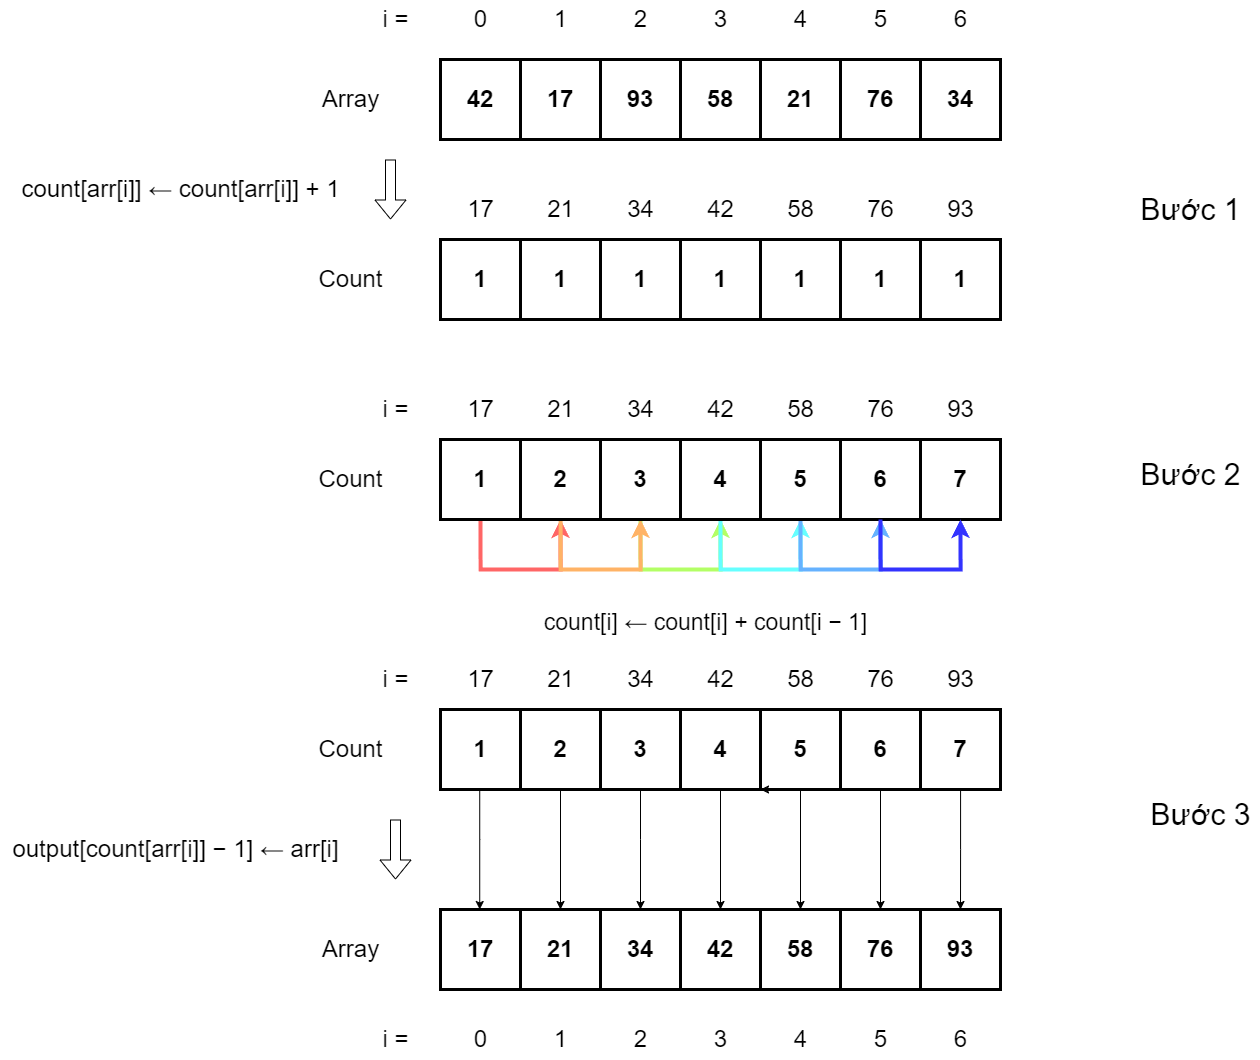
\includegraphics[width=0.75\linewidth]{img/counting_sort/1.png}
\end{figure}

\subsubsection{Độ phức tạp}

\begin{itemize}
    \item Độ phức tạp thời gian: $O(n + k)$
    \item Độ phức tạp không gian: $O(n + k)$
    \item Ưu điểm:
        \begin{itemize}
            \item Độ phức tạp thời gian tốt nhất trong các thuật toán sắp xếp: $O(n)$
            \item Không sử dụng so sánh giữa các phần tử
        \end{itemize}
    \item Nhược điểm:
    \item Ứng dụng:
        \begin{itemize}
            \item Sắp xếp các mảng có giá trị không âm và có giới hạn về giá trị của các phần tử
        \end{itemize}
\end{itemize}

